\chapter{Model selection}\label{chapter:model_selection}

Chapter \ref{chapter:robustness_assessment} explored the robustness assessment
capabilities of the PA kernel in image classification tasks, and provided extensive 
evidence of its suitability as an algorithm selection criterion in covariate shift settings. 
This chapter extends our previous findings by investigating 
how the PA kernel can be leveraged for robust epoch-wise model selection
with early stopping, potentially mitigating overfitting and enhancing
generalization performance under distribution shifts.

\section{Model selection under controled experimental conditions}\label{chapter:msel_controlled}

Building upon the exploratory results on the domain generalization setting previously obtained, 
we will assess the robust model selection capabilities of PA across a
wide range of distribution shift settings in a controlled experimental setup. In particular,
different shift factors will be considered for the source environments and also different learning
targets. These findings will help identify the experimental conditions in which the 
discriminative rationale of PA is most effective. \\

Experiments have been conducted in a setting similar to that described in Section 
\ref{results_domain_generalization}, with a reduced dataset size to avoid repetition of MNIST 
samples. This approach ensures that each training sample uniquely represents a specific instance 
of the "number drawing experiment", along with the corresponding domain 
shift perturbation. Given that shift perturbations are not entirely deterministic 
(see \texttt{diagvibsix} implementation), this approach prevents the model's inductive bias 
from being influenced by an implicit data augmentation process. \\

Both SGD and Adam optimizers under various learning rate values have been considered, 
so that the most informative results are displayed. In practice, Adam should be intuitively preferred
in this setting, as it navigates the loss landscape in a less continuous way and
explores a wider range of feature combinations, thus increasing the likelihood that domain-invariant
features are considereed for PA assessment. Nevertheless, SGD is more stable and can be used to
analyze the convergence of PA across training epochs. \\

One of the key parameters analyzed in these experiments is the shape factor of the images, which 
serves as the learning objective for the classification task. First, ERM and IRM learners are 
trained for a binary classification task involving the digit pair (1, 7), which have 
close latent representations and thus entail higher variability in learning outcomes. In this 
setting, optimal posteriors are less informative and thus agreement in the non-predicted
class is relevant for the PA penalization, as can be seen in Figure \ref{fig:modsel_17_posterior}. 
This behaviour is relevant for domain generalization, as models with similar validation accuracy 
might display different confidence levels in their
predictions and thus different generalization capabilities to unseen domains. \\

These results will be contrasted with those obtained through a 4-class classification 
involving the digits (1, 7, 4, 9). Given that (1, 7) and (4, 9) pairs are likely to be easily
discriminated, the behavior of validation accuracy should be similar to that of a binary 
classification task. However, PA is expected to discriminate both experiments and select the 
weights that better encode a domain-invariant representation by considering the whole posterior, 
not only the predicted class. An alternative experiment that considers binary classification of 
the digit pairs themselves was not pursued, as we seek a consistent inductive bias across all
the experiments presented in this work, which should be constructed only from the features 
determining each digit and the implicit contribution of shifted factors. \\

HERE PLOT OF THE POSTERIORS. \\

YOU MUST ADD A CONTROL DATASET WITH ONLY RANDOMNESS !!! \\

The characterization of the inductive bias is outside of the scope of this work, but given the
simplicity of the experimental setup and the learning task associated, it is reasonable to assume 
that it encompassess all the relevant features that are present in the data,
including the noise instantiation, the nature of the shift, and their relative frequency in the
dataset. The optimization process will iteratively navigate the loss landscape and implicitly
balance these features in a different way, leading to different predictive outcomes.  \\

In this regard, will examine two primary sources of inductive bias by varying the nature of the
shift defining environments 0 and 1, namely based on the hue factor, as was the case in the
previous chapter, and based on the position factor. These represent the two most significant 
sources of variability from an image representation perspective, and comparing the model selection 
capabilities across these settings will provide insight into the consistency of the metric. \\

The last variable to consider is the availability of target domains during validation; that is,
for model selection purposes. The domain generalization challenge requires that target domains are
inaccessible, which in our case helps select robustness-fostering algorithms from the 
vanilla ERM. Nevetheless, with the purpose of increasing the characterization of the robustness 
selection criterion, we will consider different degrees of incremental shift on the validation 
dataset, which should improve the effectiveness of the selection. \\

The last variable that will be considered is the availability of target domains during validation; 
that is, for model selection purposes. The domain generalization setting requires the assumption
that target domains are entirely inaccessible, thus discriminating robustness-fostering learners
from vanilla ERM. However, with the purpose of increasing the characterization of the robustness 
selection criterion, we will consider different degrees of incremental shift on the validation 
dataset, which should improve the effectiveness of the 
selection. Tables \ref{tab:msel_hue} and \ref{tab:msel_pos} describe the data composition of the
experiments considered. \\

HERE DATASETS. \\

NOTE THAT FIRST ENVIRONMENT IS COMMON. TAKE IT INTO ACCOUNT WHEN GIVING RESULTS. \\

- Results to show: Table with accuracy and F1 of the selected models under all conditions. 
Maybe compare validation accuracy, etc \\

- Single plot. x axis is the configuration of the validation and model selection dataset,
and y axis is the percentage of increase in performance of the accuracy-selected model With
respect to the PA-selected model. \\

It is important to note that test datasets corresponding to the first shifted factor have the same
configuration in both cases, which allows the comparison not only of different 
robustness configurations but also of algorithms that are trained to perform the same task but 
are subject to shifts of different nature.  \\

\begin{table}[H]
    \centering
    \resizebox{\textwidth}{!}{%
    \begin{tabular}{l|cl|cl|cl|cl|cl|cl}
    \multirow{2}{*}{} & \multicolumn{2}{c|}{\textbf{0}} & \multicolumn{2}{c|}{\textbf{1}} & \multicolumn{2}{c|}{\textbf{2}} & \multicolumn{2}{c|}{\textbf{3}} & \multicolumn{2}{c|}{\textbf{4}} & \multicolumn{2}{c}{\textbf{5}} \\
    \textbf{{\color{tab:blue} \textbf{ERM}}} & Acc. & $\Delta_{\operatorname{PA}}$ & Acc. & $\Delta_{\operatorname{PA}}$ & Acc. & $\Delta_{\operatorname{PA}}$ & Acc. & $\Delta_{\operatorname{PA}}$ & Acc. & $\Delta_{\operatorname{PA}}$ & Acc. & $\Delta_{\operatorname{PA}}$ \\
    \midrule
    SD & 99.4 & \PlusMinus 0.01 & 68.0 & {\color{tab:green}  \textbf{\Plus 10.1}} & 45.2 & {\color{tab:red} \textbf{\Minus 10.1}} & 42.1 & {\color{tab:red} \textbf{\Minus 6.0}} & 42.9 & {\color{tab:red} \textbf{\Minus 9.3}} & 32.0 & {\color{tab:red} \textbf{\Minus 3.8}} \\
    ID & \textbf{99.4} & \PlusMinus 0.01 & 67.1 & {\color{tab:red} \textbf{\Minus 7.9}} & 44.9 & {\color{tab:green}  \textbf{\Plus 0.8}} & 42.7 & {\color{tab:green}  \textbf{\Plus 1.3}} & 39.1 & {\color{tab:green}  \textbf{\Plus 1.5}} & 30.3 & {\color{tab:green}  \textbf{\Plus 1.4}} \\
    1F-MD & 99.4 & \PlusMinus 0.01 & 59.3 & \PlusMinus 0.01 & 46.7 & \PlusMinus 0.01 & 44.9 & \PlusMinus 0.01 & 42.5 & \PlusMinus 0.01 & 32.8 & \PlusMinus 0.01 \\
    5F-MD & 99.2 & \PlusMinus 0.01 & \textbf{74.5} & {\color{tab:red} \textbf{\Minus 13.9}} & \textbf{60.7} & {\color{tab:red} \textbf{\Minus 19.7}} & \textbf{52.9} & {\color{tab:red} \textbf{\Minus 10.0}} & \textbf{46.0} & {\color{tab:red} \textbf{\Minus 3.7}} & \textbf{38.1} & {\color{tab:red} \textbf{\Minus 1.7}} \\
    OOD & 99.2 & \PlusMinus 0.01 & 74.5 & \PlusMinus 0.01 & 60.7 & \PlusMinus 0.01 & 52.9 & \PlusMinus 0.01 & 46.0 & \PlusMinus 0.01 & 38.1 & \PlusMinus 0.01 \\
    \midrule
    \addlinespace
    \addlinespace
    \textbf{{\color{tab:orange} \textbf{IRM}}} & Acc. & $\Delta_{\operatorname{PA}}$ & Acc. & $\Delta_{\operatorname{PA}}$ & Acc. & $\Delta_{\operatorname{PA}}$ & Acc. & $\Delta_{\operatorname{PA}}$ & Acc. & $\Delta_{\operatorname{PA}}$ & Acc. & $\Delta_{\operatorname{PA}}$ \\
    \midrule
    SD & 99.4 & {\color{tab:red} \textbf{\Minus 0.2}} & 77.0 & {\color{tab:green}  \textbf{\Plus 3.2}} & 34.7 & {\color{tab:green}  \textbf{\Plus 5.5}} & 39.5 & {\color{tab:green}  \textbf{\Plus 2.3}} & 42.0 & {\color{tab:green}  \textbf{\Plus 1.9}} & 29.1 & {\color{tab:green}  \textbf{\Plus 2.4}} \\
    ID & \textbf{99.4} & {\color{tab:red} \textbf{\Minus 0.2}} & 71.2 & {\color{tab:green}  \textbf{\Plus 12.6}} & \textbf{51.2} & {\color{tab:red} \textbf{\Minus 0.8}} & \textbf{55.1} & {\color{tab:green}  \textbf{\Plus 0.1}} & \textbf{52.8} & {\color{tab:red} \textbf{\Minus 1.5}} & \textbf{38.4} & {\color{tab:red} \textbf{\Minus 1.3}} \\
    1F-MD & 99.2 & \PlusMinus 0.01 & \textbf{80.2} & \PlusMinus 0.01 & 40.2 & \PlusMinus 0.01 & 41.8 & \PlusMinus 0.01 & 43.9 & \PlusMinus 0.01 & 31.5 & \PlusMinus 0.01 \\
    5F-MD & 99.4 & {\color{tab:red} \textbf{\Minus 0.7}} & 71.2 & {\color{tab:red} \textbf{\Minus 14.8}} & 51.2 & {\color{tab:green}  \textbf{\Plus 4.8}} & 55.1 & {\color{tab:red} \textbf{\Minus 1.8}} & 52.8 & {\color{tab:red} \textbf{\Minus 6.8}} & 38.4 & {\color{tab:red} \textbf{\Minus 8.1}} \\
    OOD & 99.2 & \PlusMinus 0.01 & 69.1 & \PlusMinus 0.01 & 46.3 & \PlusMinus 0.01 & 49.4 & \PlusMinus 0.01 & 46.6 & \PlusMinus 0.01 & 31.8 & \PlusMinus 0.01 \\
    \bottomrule
    \end{tabular}%
    }
    \caption{REMOVEopt=adam-lr=0.0001-mf=hue-npair=FalseREMOVE Test performance on increasingly shifted datasets for models selected during ERM and IRM procedures. Different validation datasets are used, and the selection capabilities of PA and validation accuracy are compared.}
    \label{tab:label}
    \end{table}
    
    \begin{table}[H]
    \centering
    \resizebox{\textwidth}{!}{%
    \begin{tabular}{l|cl|cl|cl|cl|cl|cl}
    \multirow{2}{*}{} & \multicolumn{2}{c|}{\textbf{0}} & \multicolumn{2}{c|}{\textbf{1}} & \multicolumn{2}{c|}{\textbf{2}} & \multicolumn{2}{c|}{\textbf{3}} & \multicolumn{2}{c|}{\textbf{4}} & \multicolumn{2}{c}{\textbf{5}} \\
    \textbf{{\color{tab:blue} \textbf{ERM}}} & Acc. & $\Delta_{\operatorname{PA}}$ & Acc. & $\Delta_{\operatorname{PA}}$ & Acc. & $\Delta_{\operatorname{PA}}$ & Acc. & $\Delta_{\operatorname{PA}}$ & Acc. & $\Delta_{\operatorname{PA}}$ & Acc. & $\Delta_{\operatorname{PA}}$ \\
    \midrule
    SD & \textbf{99.4} & {\color{tab:red} \textbf{\Minus 0.1}} & 59.3 & {\color{tab:green}  \textbf{\Plus 8.3}} & 46.7 & {\color{tab:green}  \textbf{\Plus 1.5}} & 44.9 & {\color{tab:green}  \textbf{\Plus 1.5}} & 42.5 & {\color{tab:green}  \textbf{\Plus 0.9}} & 32.8 & {\color{tab:red} \textbf{\Minus 1.5}} \\
    ID & 99.4 & {\color{tab:red} \textbf{\Minus 0.1}} & 59.3 & {\color{tab:green}  \textbf{\Plus 8.3}} & 46.7 & {\color{tab:green}  \textbf{\Plus 1.5}} & 44.9 & {\color{tab:green}  \textbf{\Plus 1.5}} & 42.5 & {\color{tab:green}  \textbf{\Plus 0.9}} & 32.8 & {\color{tab:red} \textbf{\Minus 1.5}} \\
    1F-MD & 99.4 & \PlusMinus 0.01 & 59.3 & \PlusMinus 0.01 & 46.7 & \PlusMinus 0.01 & 44.9 & \PlusMinus 0.01 & 42.5 & \PlusMinus 0.01 & 32.8 & \PlusMinus 0.01 \\
    5F-MD & 99.2 & \PlusMinus 0.01 & \textbf{74.5} & {\color{tab:red} \textbf{\Minus 13.9}} & \textbf{60.7} & {\color{tab:red} \textbf{\Minus 19.7}} & \textbf{52.9} & {\color{tab:red} \textbf{\Minus 10.0}} & \textbf{46.0} & {\color{tab:red} \textbf{\Minus 3.7}} & \textbf{38.1} & {\color{tab:red} \textbf{\Minus 1.7}} \\
    OOD & 99.2 & \PlusMinus 0.01 & 74.5 & \PlusMinus 0.01 & 60.7 & \PlusMinus 0.01 & 52.9 & \PlusMinus 0.01 & 46.0 & \PlusMinus 0.01 & 38.1 & \PlusMinus 0.01 \\
    \midrule
    \addlinespace
    \addlinespace
    \textbf{{\color{tab:orange} \textbf{IRM}}} & Acc. & $\Delta_{\operatorname{PA}}$ & Acc. & $\Delta_{\operatorname{PA}}$ & Acc. & $\Delta_{\operatorname{PA}}$ & Acc. & $\Delta_{\operatorname{PA}}$ & Acc. & $\Delta_{\operatorname{PA}}$ & Acc. & $\Delta_{\operatorname{PA}}$ \\
    \midrule
    SD & \textbf{99.4} & \PlusMinus 0.01 & 74.4 & {\color{tab:red} \textbf{\Minus 4.7}} & 41.4 & {\color{tab:green}  \textbf{\Plus 14.2}} & 43.8 & {\color{tab:green}  \textbf{\Plus 14.5}} & 41.6 & {\color{tab:green}  \textbf{\Plus 14.9}} & 26.9 & {\color{tab:green}  \textbf{\Plus 11.5}} \\
    ID & 99.3 & {\color{tab:red} \textbf{\Minus 0.2}} & 81.9 & {\color{tab:red} \textbf{\Minus 12.9}} & 52.4 & {\color{tab:red} \textbf{\Minus 6.1}} & 54.5 & {\color{tab:red} \textbf{\Minus 5.1}} & 54.1 & {\color{tab:red} \textbf{\Minus 7.6}} & 36.5 & {\color{tab:red} \textbf{\Minus 4.7}} \\
    1F-MD & 99.2 & \PlusMinus 0.01 & 80.2 & \PlusMinus 0.01 & 40.2 & \PlusMinus 0.01 & 41.8 & \PlusMinus 0.01 & 43.9 & \PlusMinus 0.01 & 31.5 & \PlusMinus 0.01 \\
    5F-MD & 99.4 & \PlusMinus 0.01 & \textbf{84.1} & {\color{tab:red} \textbf{\Minus 2.0}} & \textbf{54.3} & {\color{tab:red} \textbf{\Minus 3.2}} & \textbf{56.3} & {\color{tab:red} \textbf{\Minus 2.0}} & \textbf{54.7} & {\color{tab:red} \textbf{\Minus 0.8}} & \textbf{38.3} & {\color{tab:red} \textbf{\Minus 1.1}} \\
    OOD & 99.2 & \PlusMinus 0.01 & 69.1 & \PlusMinus 0.01 & 46.3 & \PlusMinus 0.01 & 49.4 & \PlusMinus 0.01 & 46.6 & \PlusMinus 0.01 & 31.8 & \PlusMinus 0.01 \\
    \bottomrule
    \end{tabular}%
    }
    \caption{REMOVEopt=adam-lr=0.0001-mf=hue-npair=TrueREMOVE Test performance on increasingly shifted datasets for models selected during ERM and IRM procedures. Different validation datasets are used, and the selection capabilities of PA and validation accuracy are compared.}
    \label{tab:label}
    \end{table}
    
    \begin{table}[H]
    \centering
    \resizebox{\textwidth}{!}{%
    \begin{tabular}{l|cl|cl|cl|cl|cl|cl}
    \multirow{2}{*}{} & \multicolumn{2}{c|}{\textbf{0}} & \multicolumn{2}{c|}{\textbf{1}} & \multicolumn{2}{c|}{\textbf{2}} & \multicolumn{2}{c|}{\textbf{3}} & \multicolumn{2}{c|}{\textbf{4}} & \multicolumn{2}{c}{\textbf{5}} \\
    \textbf{{\color{tab:blue} \textbf{ERM}}} & Acc. & $\Delta_{\operatorname{PA}}$ & Acc. & $\Delta_{\operatorname{PA}}$ & Acc. & $\Delta_{\operatorname{PA}}$ & Acc. & $\Delta_{\operatorname{PA}}$ & Acc. & $\Delta_{\operatorname{PA}}$ & Acc. & $\Delta_{\operatorname{PA}}$ \\
    \midrule
    ID & 99.3 & {\color{tab:green}  \textbf{\Plus 0.2}} & 99.4 & {\color{tab:green}  \textbf{\Plus 0.2}} & 86.6 & {\color{tab:red} \textbf{\Minus 1.3}} & \textbf{68.5} & {\color{tab:green}  \textbf{\Plus 5.7}} & 50.8 & {\color{tab:green}  \textbf{\Plus 4.0}} & 47.4 & {\color{tab:green}  \textbf{\Plus 8.2}} \\
    1F-MD & \textbf{99.3} & {\color{tab:red} \textbf{\Minus 0.1}} & \textbf{99.5} & {\color{tab:red} \textbf{\Minus 0.1}} & 84.9 & {\color{tab:green}  \textbf{\Plus 4.0}} & 66.3 & {\color{tab:green}  \textbf{\Plus 1.8}} & 52.0 & {\color{tab:green}  \textbf{\Plus 1.6}} & 46.3 & {\color{tab:green}  \textbf{\Plus 7.4}} \\
    5F-MD & 99.2 & \PlusMinus 0.01 & 99.3 & {\color{tab:green}  \textbf{\Plus 0.1}} & 80.9 & {\color{tab:green}  \textbf{\Plus 3.8}} & 64.5 & {\color{tab:red} \textbf{\Minus 0.8}} & \textbf{66.8} & {\color{tab:green}  \textbf{\Plus 2.8}} & \textbf{58.3} & {\color{tab:red} \textbf{\Minus 1.3}} \\
    OOD & 99.3 & {\color{tab:green}  \textbf{\Plus 0.1}} & 99.4 & \PlusMinus 0.01 & \textbf{89.0} & {\color{tab:red} \textbf{\Minus 4.7}} & 68.0 & {\color{tab:red} \textbf{\Minus 7.6}} & 53.6 & {\color{tab:red} \textbf{\Minus 6.7}} & 53.6 & {\color{tab:red} \textbf{\Minus 8.7}} \\
    \midrule
    \addlinespace
    \addlinespace
    \textbf{{\color{tab:orange} \textbf{IRM}}} & Acc. & $\Delta_{\operatorname{PA}}$ & Acc. & $\Delta_{\operatorname{PA}}$ & Acc. & $\Delta_{\operatorname{PA}}$ & Acc. & $\Delta_{\operatorname{PA}}$ & Acc. & $\Delta_{\operatorname{PA}}$ & Acc. & $\Delta_{\operatorname{PA}}$ \\
    \midrule
    ID & \textbf{99.4} & {\color{tab:red} \textbf{\Minus 0.2}} & \textbf{99.5} & {\color{tab:red} \textbf{\Minus 0.1}} & 86.4 & {\color{tab:red} \textbf{\Minus 3.5}} & 50.4 & {\color{tab:green}  \textbf{\Plus 12.0}} & 48.2 & {\color{tab:green}  \textbf{\Plus 22.2}} & 39.8 & {\color{tab:green}  \textbf{\Plus 19.8}} \\
    1F-MD & 99.4 & \PlusMinus 0.01 & 99.5 & \PlusMinus 0.01 & 86.5 & {\color{tab:green}  \textbf{\Plus 0.1}} & 50.7 & {\color{tab:red} \textbf{\Minus 4.1}} & 48.3 & {\color{tab:green}  \textbf{\Plus 0.6}} & 39.0 & {\color{tab:red} \textbf{\Minus 3.1}} \\
    5F-MD & 99.2 & \PlusMinus 0.01 & 99.5 & \PlusMinus 0.01 & 83.0 & \PlusMinus 0.01 & \textbf{62.4} & \PlusMinus 0.01 & \textbf{70.4} & \PlusMinus 0.01 & \textbf{59.6} & \PlusMinus 0.01 \\
    OOD & 99.4 & \PlusMinus 0.01 & 99.5 & \PlusMinus 0.01 & \textbf{86.6} & \PlusMinus 0.01 & 46.5 & \PlusMinus 0.01 & 48.8 & \PlusMinus 0.01 & 35.9 & \PlusMinus 0.01 \\
    \bottomrule
    \end{tabular}%
    }
    \caption{REMOVEopt=adam-lr=0.0001-mf=pos-npair=FalseREMOVE Test performance on increasingly shifted datasets for models selected during ERM and IRM procedures. Different validation datasets are used, and the selection capabilities of PA and validation accuracy are compared.}
    \label{tab:label}
    \end{table}
    
    \begin{table}[H]
    \centering
    \resizebox{\textwidth}{!}{%
    \begin{tabular}{l|cl|cl|cl|cl|cl|cl}
    \multirow{2}{*}{} & \multicolumn{2}{c|}{\textbf{0}} & \multicolumn{2}{c|}{\textbf{1}} & \multicolumn{2}{c|}{\textbf{2}} & \multicolumn{2}{c|}{\textbf{3}} & \multicolumn{2}{c|}{\textbf{4}} & \multicolumn{2}{c}{\textbf{5}} \\
    \textbf{{\color{tab:blue} \textbf{ERM}}} & Acc. & $\Delta_{\operatorname{PA}}$ & Acc. & $\Delta_{\operatorname{PA}}$ & Acc. & $\Delta_{\operatorname{PA}}$ & Acc. & $\Delta_{\operatorname{PA}}$ & Acc. & $\Delta_{\operatorname{PA}}$ & Acc. & $\Delta_{\operatorname{PA}}$ \\
    \midrule
    SD & 99.4 & {\color{tab:red} \textbf{\Minus 0.2}} & \textbf{99.5} & {\color{tab:red} \textbf{\Minus 0.1}} & 78.6 & {\color{tab:green}  \textbf{\Plus 8.1}} & \textbf{77.3} & {\color{tab:red} \textbf{\Minus 13.2}} & 36.7 & {\color{tab:green}  \textbf{\Plus 13.3}} & 38.1 & {\color{tab:green}  \textbf{\Plus 13.7}} \\
    ID & 99.3 & {\color{tab:green}  \textbf{\Plus 0.1}} & 99.5 & {\color{tab:red} \textbf{\Minus 0.1}} & 84.9 & {\color{tab:green}  \textbf{\Plus 1.6}} & 66.3 & {\color{tab:green}  \textbf{\Plus 2.7}} & 52.0 & {\color{tab:red} \textbf{\Minus 1.7}} & 46.3 & {\color{tab:green}  \textbf{\Plus 1.8}} \\
    1F-MD & 99.3 & {\color{tab:green}  \textbf{\Plus 0.1}} & 99.5 & {\color{tab:red} \textbf{\Minus 0.1}} & 84.9 & {\color{tab:green}  \textbf{\Plus 1.6}} & 66.3 & {\color{tab:green}  \textbf{\Plus 2.7}} & 52.0 & {\color{tab:red} \textbf{\Minus 1.7}} & 46.3 & {\color{tab:green}  \textbf{\Plus 1.8}} \\
    5F-MD & 99.4 & \PlusMinus 0.01 & 99.5 & \PlusMinus 0.01 & \textbf{87.4} & \PlusMinus 0.01 & 74.5 & \PlusMinus 0.01 & 56.4 & {\color{tab:red} \textbf{\Minus 0.1}} & \textbf{57.6} & \PlusMinus 0.01 \\
    OOD & \textbf{99.5} & \PlusMinus 0.01 & 99.5 & {\color{tab:red} \textbf{\Minus 0.1}} & 87.0 & {\color{tab:red} \textbf{\Minus 0.5}} & 75.1 & {\color{tab:red} \textbf{\Minus 6.1}} & \textbf{56.9} & {\color{tab:red} \textbf{\Minus 6.7}} & 57.5 & {\color{tab:red} \textbf{\Minus 9.4}} \\
    \midrule
    \addlinespace
    \addlinespace
    \textbf{{\color{tab:orange} \textbf{IRM}}} & Acc. & $\Delta_{\operatorname{PA}}$ & Acc. & $\Delta_{\operatorname{PA}}$ & Acc. & $\Delta_{\operatorname{PA}}$ & Acc. & $\Delta_{\operatorname{PA}}$ & Acc. & $\Delta_{\operatorname{PA}}$ & Acc. & $\Delta_{\operatorname{PA}}$ \\
    \midrule
    SD & \textbf{99.4} & {\color{tab:red} \textbf{\Minus 0.1}} & 99.4 & {\color{tab:green}  \textbf{\Plus 0.1}} & \textbf{86.2} & {\color{tab:red} \textbf{\Minus 8.5}} & 51.1 & {\color{tab:green}  \textbf{\Plus 6.3}} & 48.9 & {\color{tab:green}  \textbf{\Plus 7.0}} & 38.6 & {\color{tab:green}  \textbf{\Plus 11.9}} \\
    ID & 99.3 & \PlusMinus 0.01 & \textbf{99.5} & \PlusMinus 0.01 & 77.7 & \PlusMinus 0.01 & 57.4 & \PlusMinus 0.01 & 55.9 & \PlusMinus 0.01 & 50.4 & \PlusMinus 0.01 \\
    1F-MD & 99.3 & {\color{tab:red} \textbf{\Minus 0.1}} & 99.5 & \PlusMinus 0.01 & 84.6 & {\color{tab:red} \textbf{\Minus 6.9}} & \textbf{69.8} & {\color{tab:red} \textbf{\Minus 12.4}} & 64.4 & {\color{tab:red} \textbf{\Minus 8.5}} & 57.5 & {\color{tab:red} \textbf{\Minus 7.1}} \\
    5F-MD & 99.2 & \PlusMinus 0.01 & 99.5 & \PlusMinus 0.01 & 83.0 & \PlusMinus 0.01 & 62.4 & \PlusMinus 0.01 & \textbf{70.4} & \PlusMinus 0.01 & \textbf{59.6} & \PlusMinus 0.01 \\
    OOD & 99.3 & \PlusMinus 0.01 & 99.5 & \PlusMinus 0.01 & 84.6 & \PlusMinus 0.01 & 69.8 & \PlusMinus 0.01 & 64.4 & \PlusMinus 0.01 & 57.5 & \PlusMinus 0.01 \\
    \bottomrule
    \end{tabular}%
    }
    \caption{REMOVEopt=adam-lr=0.0001-mf=pos-npair=TrueREMOVE Test performance on increasingly shifted datasets for models selected during ERM and IRM procedures. Different validation datasets are used, and the selection capabilities of PA and validation accuracy are compared.}
    \label{tab:label}
    \end{table}

\section{ID model selection}

In the preceding chapters, evidence was provided supporting PA as a suitable robustness metric 
that effectively captures generalization capabilities under both sampling randomness and 
covariate shift. So far, experiments in the domain generalization setting have been conducted 
under synthetic conditions in which distribution shift is the only accountable source of randomenss 
between  $\bm{x}$ and $\bm{x}^{\prime \prime}$. These experiments have shown that PA successfully 
discriminates robust from non-robust learners and also provides increased early-stopping performance compared with
current baseline metrics. \\

However, real-world datasets are subject to sampling randomness and often exhibit feature
distributions that are severely misaligned with the true distribution in the sample space, 
which is commonly known as subpopulation shift. This section aims to reproduce these conditions 
by considering controlled environments where the presence of certain image factors is deliberately 
manipulated to induce an inductive bias towards suboptimal representations. These representations 
may generalize well to sampling variability within source environments but fail to adapt to 
distributional shifts in target environments, which poses an additional challenge to
our domain generalization problem. \\

Epoch-wise model selection under these conditions entails a fundamentally different approach,
especially regarding experiments performed in the previous chapter. Evaluating PA on a model
selected by performance standards (i.e. validation accuracy) and 

- Here interpretation of the validation accuracy.

- The datasets should be explained maybe. \\


\begin{definition}[SO/GO in DiagVib-6]\label{def:zso_theory}
    Let shape, hue, lightness, position, scale and texture be MNIST image factors that can be manipulated
    throught the DiagViB-6 data generation pipeline. Let $F^P$ be the factor to be predicted by the 
    classifier, and $F^L$ the factor taking different values in the training and validation datasets,
    thus defining source environments. \\
    
    The inductive bias of the model will be influenced by
    spurious correlations between $F^P$ and $F^L$ if the co-occurrence of their instances is
    not uniform \cite{euligDiagViB6DiagnosticBenchmark2021}. From that perspective, 
    a shortcut opportunity (SO) will be induced when a specific instance of $F^P$ is exclusively co-occurrent with a specific instance of $F^L$.
    Conversely, a generalization opportunity (GO) will arise when such $F^P$ and $F^L$ instances
    are each additionally co-occurrent with other instances of $F^L$ and $F^P$, respectively, thus breaking
    the exclusivity. In this work, we will consider three particular settings:

    \begin{itemize}
        \item Zero generalization opportunities (ZGO): Each instance of $F^P$ is exclusively co-occurrent with a 
        unique instance of $F^L$. The model is expected to overfit to spurious correlations and thus generalize
        poorly to datasets in which these are not present.
        \item Compositional generalization opportunities (CGO): Starting from the ZGO setting, the exclusive co-occurrence
        between some instances of $F^P$ and $F^L$ is broken by the presence of generalization opportunities. The model 
        should be increasingly robust to unseen combinations the higher is the number of generalization opportunities.
        \item Zero shortcut opportunities (ZSO): All instances of $F^P$ are uniformly co-occurrent with all 
        instances of $F^L$, so that all combinations of factors are present in source domains.
    \end{itemize}

    The setting for ID model selection requires that validation datasets contain the
    same configuration of factors than the training datasets. Experiments will be performed for
    ZGO, ZSO and single, double and triple CGO.

    \begin{figure}[H]
        \centering
        % LEGEND
        \begin{subfigure}[b]{\textwidth}
            \centering
            % Here, you would include your legend, for example, a dummy image
            
\includegraphics[width=0.6\textwidth]{img/datasets/_legend_theory.pdf}
        \end{subfigure}
        \vspace{-0.2cm} % Add some vertical space between the legend and the subfigures

        \begin{subfigure}[b]{0.17\textwidth}
            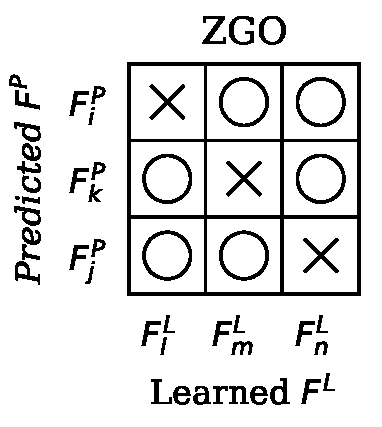
\includegraphics[width=\textwidth]{img/datasets/_ZGO.pdf}
        \end{subfigure}
        \hfill
        \begin{subfigure}[b]{0.17\textwidth}
            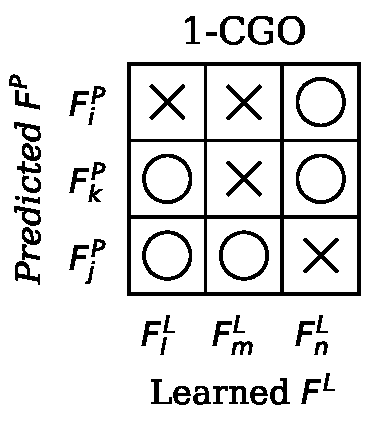
\includegraphics[width=\textwidth]{img/datasets/_1-CGO.pdf}
        \end{subfigure}
        \hfill
        \begin{subfigure}[b]{0.17\textwidth}
            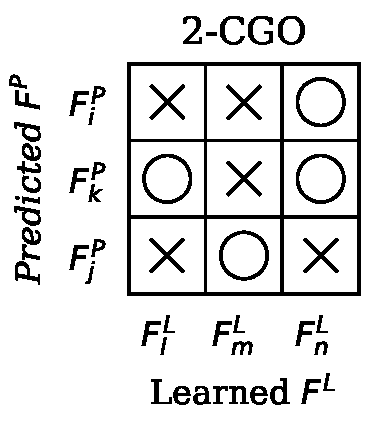
\includegraphics[width=\textwidth]{img/datasets/_2-CGO.pdf}
        \end{subfigure}
        \hfill
        \begin{subfigure}[b]{0.17\textwidth}
            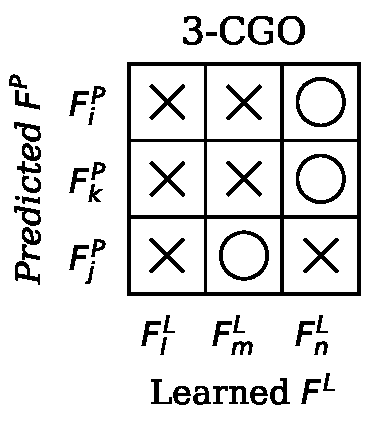
\includegraphics[width=\textwidth]{img/datasets/_3-CGO.pdf}
        \end{subfigure}
        \hfill
        \begin{subfigure}[b]{0.17\textwidth}
            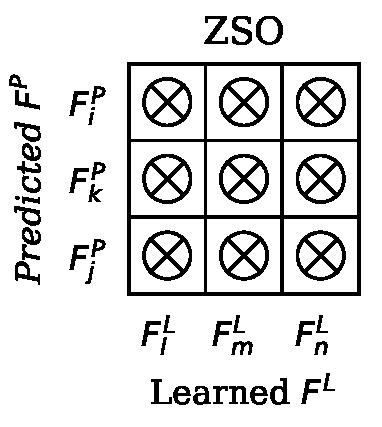
\includegraphics[width=\textwidth]{img/datasets/_ZSO.pdf}
        \end{subfigure}
        
        \caption{Blabla...}
    \end{figure}
\end{definition}




can be used as an early stopping criterion
for model selection. Nevertheless, real world applications do not usually have a 



More especifically,
we aim at characterizing the response of the metric under different variations in the inductive
bias of the model, which implicitly shifts according to the availability of certain features
in the data. In this regard, two 

1. Why epochwise is different than general model selection. KEY: Validation accuracy. The
main problem in any robustness measurement is that we are not able to distinguish sampling
randomness from robustness to adversarial shifts


2. We want to explore the difference between validation accuracy and PA for different inductive
bias.

Best optimization hyperparameters were selected so that the
best accuracy performance was obtained. No complex heuristic was
needed given that the best hyperparameters were also the best
for both learnes and for all datasets with very few exceptions.
Otherwise select the highest on the first domain, as the other
domains are less significant. 
For that reason, odels in the same table contain the same hyperparameters. \\

REMOVE ENV 1 FOR ZSO \\

3. Results show that. What we do is paired because we want to make sure that
the model overfits to the domains. \\

\begin{table}[H]
    \centering
    \resizebox{\textwidth}{!}{%
    \begin{tabular}{l|cl|cl|cl|cl|cl|cl}
    \multirow{2}{*}{} & \multicolumn{2}{c|}{\textbf{0}} & \multicolumn{2}{c|}{\textbf{1}} & \multicolumn{2}{c|}{\textbf{2}} & \multicolumn{2}{c|}{\textbf{3}} & \multicolumn{2}{c|}{\textbf{4}} & \multicolumn{2}{c}{\textbf{5}} \\
    \textbf{{\color{tab:blue} \textbf{ERM}}} & Acc. & $\Delta_{\operatorname{PA}}$ & Acc. & $\Delta_{\operatorname{PA}}$ & Acc. & $\Delta_{\operatorname{PA}}$ & Acc. & $\Delta_{\operatorname{PA}}$ & Acc. & $\Delta_{\operatorname{PA}}$ & Acc. & $\Delta_{\operatorname{PA}}$ \\
    \midrule
    ZGO & 99.9 & {\color{tab:red} \textbf{\Minus 45.6}} & 30.4 & {\color{tab:green}  \textbf{\Plus 4.0}} & 33.3 & {\color{tab:green}  \textbf{\Plus 2.4}} & 28.8 & {\color{tab:red} \textbf{\Minus 0.3}} & 33.6 & {\color{tab:red} \textbf{\Minus 0.3}} & 33.4 & {\color{tab:green}  \textbf{\Plus 1.4}} \\
    1-CGO & 99.4 & {\color{tab:red} \textbf{\Minus 51.8}} & 23.5 & {\color{tab:green}  \textbf{\Plus 5.1}} & 25.1 & {\color{tab:green}  \textbf{\Plus 4.0}} & 14.8 & {\color{tab:green}  \textbf{\Plus 13.5}} & 32.7 & {\color{tab:red} \textbf{\Minus 2.4}} & 33.4 & {\color{tab:red} \textbf{\Minus 2.3}} \\
    2-CGO & 98.5 & \PlusMinus 0.01 & 57.5 & \PlusMinus 0.01 & 58.3 & \PlusMinus 0.01 & 37.1 & \PlusMinus 0.01 & 38.9 & \PlusMinus 0.01 & 38.5 & \PlusMinus 0.01 \\
    3-CGO & 98.3 & \PlusMinus 0.01 & 65.7 & \PlusMinus 0.01 & 66.0 & \PlusMinus 0.01 & 42.8 & \PlusMinus 0.01 & 41.8 & \PlusMinus 0.01 & 40.3 & \PlusMinus 0.01 \\
    ZSO & 97.8 & \PlusMinus 0.01 & 97.7 & \PlusMinus 0.01 & 65.5 & \PlusMinus 0.01 & 44.4 & \PlusMinus 0.01 & 43.5 & \PlusMinus 0.01 & 43.7 & \PlusMinus 0.01 \\
    \midrule
    \addlinespace
    \addlinespace
    \textbf{{\color{tab:orange} \textbf{IRM}}} & Acc. & $\Delta_{\operatorname{PA}}$ & Acc. & $\Delta_{\operatorname{PA}}$ & Acc. & $\Delta_{\operatorname{PA}}$ & Acc. & $\Delta_{\operatorname{PA}}$ & Acc. & $\Delta_{\operatorname{PA}}$ & Acc. & $\Delta_{\operatorname{PA}}$ \\
    \midrule
    ZGO & 100.0 & {\color{tab:red} \textbf{\Minus 32.9}} & 30.2 & {\color{tab:green}  \textbf{\Plus 5.4}} & 33.9 & {\color{tab:green}  \textbf{\Plus 1.9}} & 28.3 & {\color{tab:green}  \textbf{\Plus 4.0}} & 32.6 & {\color{tab:green}  \textbf{\Plus 1.0}} & 32.7 & {\color{tab:green}  \textbf{\Plus 2.3}} \\
    1-CGO & 99.6 & {\color{tab:red} \textbf{\Minus 40.0}} & 22.7 & {\color{tab:green}  \textbf{\Plus 2.3}} & 24.8 & {\color{tab:green}  \textbf{\Plus 1.7}} & 10.7 & {\color{tab:green}  \textbf{\Plus 17.9}} & 32.9 & {\color{tab:red} \textbf{\Minus 3.9}} & 33.4 & {\color{tab:red} \textbf{\Minus 2.2}} \\
    2-CGO & 98.9 & {\color{tab:red} \textbf{\Minus 0.1}} & 59.2 & {\color{tab:red} \textbf{\Minus 0.6}} & 57.7 & {\color{tab:red} \textbf{\Minus 0.2}} & 40.5 & {\color{tab:red} \textbf{\Minus 0.4}} & 39.2 & {\color{tab:red} \textbf{\Minus 0.3}} & 38.3 & {\color{tab:red} \textbf{\Minus 0.1}} \\
    3-CGO & 98.5 & \PlusMinus 0.01 & 67.7 & \PlusMinus 0.01 & 67.7 & \PlusMinus 0.01 & 45.5 & \PlusMinus 0.01 & 43.1 & \PlusMinus 0.01 & 41.9 & \PlusMinus 0.01 \\
    ZSO & 98.5 & \PlusMinus 0.01 & 98.2 & \PlusMinus 0.01 & 68.4 & \PlusMinus 0.01 & 46.6 & \PlusMinus 0.01 & 45.2 & \PlusMinus 0.01 & 45.4 & \PlusMinus 0.01 \\
    \bottomrule
    \end{tabular}%
    }
    \caption{REMOVEopt=sgd-lr=0.0001-mf=hue-npair=FalseREMOVE Test performance on increasingly shifted datasets for models selected during ERM and IRM procedures. Different validation datasets are used, and the selection capabilities of PA and validation accuracy are compared.}
    \label{tab:label}
    \end{table}



If the goal is to show that it performs better than accuracy, that can be easily shown, but the improvement is non-significative.
. But the principal challenge is theoretical: real-world covariate shift encompasses both distribution shift and sampling randomness, and PA (in the way we have been handling it) does not distinguish between them. When we compare the evolution of the training in between epochs, we will select the most robust features, but they won't necessarily be the most generalizable ones, they will depend on the nature of the data.
=> Here follows experiments on GO/SO. Explain the conclusions derived by those experiments.
    1) Even when features are very similar, PA keeps increasing.
    2) Model with more generalization opportunities is the least robust in high-shift scenarios. THIS IS THE KEY. The fact that robustness is so disentangled from accuracy (cite theoretical properties again) turns against us because what we want is actually to perform good. The reason is that SO entail a reduction in the effective feature space that the model navigates, which makes it more robust by definition.
=> Show the simple GO/SO experiment with paired samples. No sampling noise between X' and X'', only distribution shift.
. Alternative way of thinking about it is forgetting about images. We are comparing different models
 trained on different instantiations of the features that represent our data. The randomness 
 associated with the sampling process does not present homeocedasticity, as noise magnitude 
 increases with the distance between domains. The more generalizable, the more room for variation. 
 In such case, PA would select the best model when the goal is to make features converge. In some 
 sense it is, but overfitting to examples or subpopulation shifts would yield the same response.

 For instance, I try to justify why PA does not always select the best performing model by reformulating the problem so that the inputs are image features rather than images themselves. Every epoch represents an instantiation of the "feature extraction" experiment, and in such case a model overfitting to the shortcut opportunities in the data is also considered robust, since we don't control how much of the robustness "value" is attributed to sampling randomness and how much to the distribution shift. Sampling randomness can be modelled with the taus, and the key is that it presents heterocedasticity, in the sense that its "spread" is reduced when the model learns (also if it learns the wrong features) and that affects the PA value.

 The most "elegant" way I have been able to devise (in the sense that it compiles both a measure of sampling noise and a measure of distribution shift) is comparing the first PCA direction in the feature space between both environments. The spread of each label in the PCA direction accounts for sampling randomness, whereas the MSE between components of the same sample in different environments accounts for distribution shift.

 \section{Model selection on benchmark datasets}

In light of the results obtained in the previous sections, we will finally assess the model selection
capabilities of PA on benchmark datasets. In particular, several WILDS 
\cite{kohWILDSBenchmarkIntheWild2021} datasets will be considered, as they provide a comprehensive
set of domain generalization tasks that are representative of real-world scenarios. Each of the
datasets under consideration entails a specific configuration of learning opportunities that will
shift the inductive bias towards suboptimal representations for out-of-distribution
generalization. The performance displayed by PA in the previous chapter will be considered when
evaluating its behaviour under these conditions.\\


 - Show plot of the posteriors for each dataset. \\
 - Show table with results on model selection. \\

 \cleardoublepage